\section{INTRODUCTION}
Recent researches on Vertical Take Off and Landing (VTOL) systems have shown interest on both \emph{passive} (e.g., inspection and remote sensing) and \emph{active} tasks (e.g., grasping and manipulation). The dexterity required for achieving the latter often calls for the design of complex-shaped aerial vehicles with several Degrees of Freedom (DoF), which complicate the control design \cite{c8}\cite{c9}\cite{c10}. 

Additionally, when the VTOL needs to operate in outdoor environments, the control design is further complicated by the environment uncertainties, e.g. the aerodynamic effects that arise in presence of wind and while the vehicle is performing high speed movements \cite{c11}\cite{c13}. In this paper, we propose a simple yet effective modeling and control strategy to handle these aerodynamic effects on a complex-shaped, high DoF VTOL system: a jet-powered humanoid robot.

% One of the major problems in developing flight control systems of UAVs is modeling uncertainties and parameter variations in characterizing the vehicle and its operating environment \cite{c11}\cite{c13}. The underactuated Vertical Take-Off and Landing (VTOL) UAVs which are often subject to disturbances caused by non-modeled external effects and other have attracted the effort from the nonlinear control community \cite{c1}. 
%
%This paper takes a step on modeling aerodynamic effects acting on complex-shaped and underactuated VTOLs operating in critical environments (e.g. wind gust) based on Computational Fluid Dynamics  (CFD) analysis, moreover, control techniques towards aerodynamic effects are developed to stabilize the robot or improve the performance.


%----------------------------------------------------------%

The combination of terrestrial and aerial locomotion in a single robotic platform is of some interest in the robotics community, which recently proposed hexapod-quadrotor designs, hybrid terrestrials and aerial quadrotors, insect biobots, and humanoid robots with thrusters \cite{pitonyak2017hexapod}\cite{kalantari2013hytaq}\cite{bozkurt2009insectbio}\cite{LeoCaltech}\cite{Jet-HR1}. An attempt to unify manipulation, aerial, and bipedal terrestrial locomotion on a single robotic platform is being carried out by the iRonCub project~\cite{Bartolozzi2017iCubTN}\cite{c1}\cite{c2}. As shown in Fig. \ref{fig:iron_cad}, four jet engines located on the robot arms and chest are used to lift the robot from the ground. The increased operativity and mobility of this type of platforms, however, often come at the cost of a complex-shaped hardware design with numerous DoF.\looseness=-1

\begin{figure}[t]
      \centering
      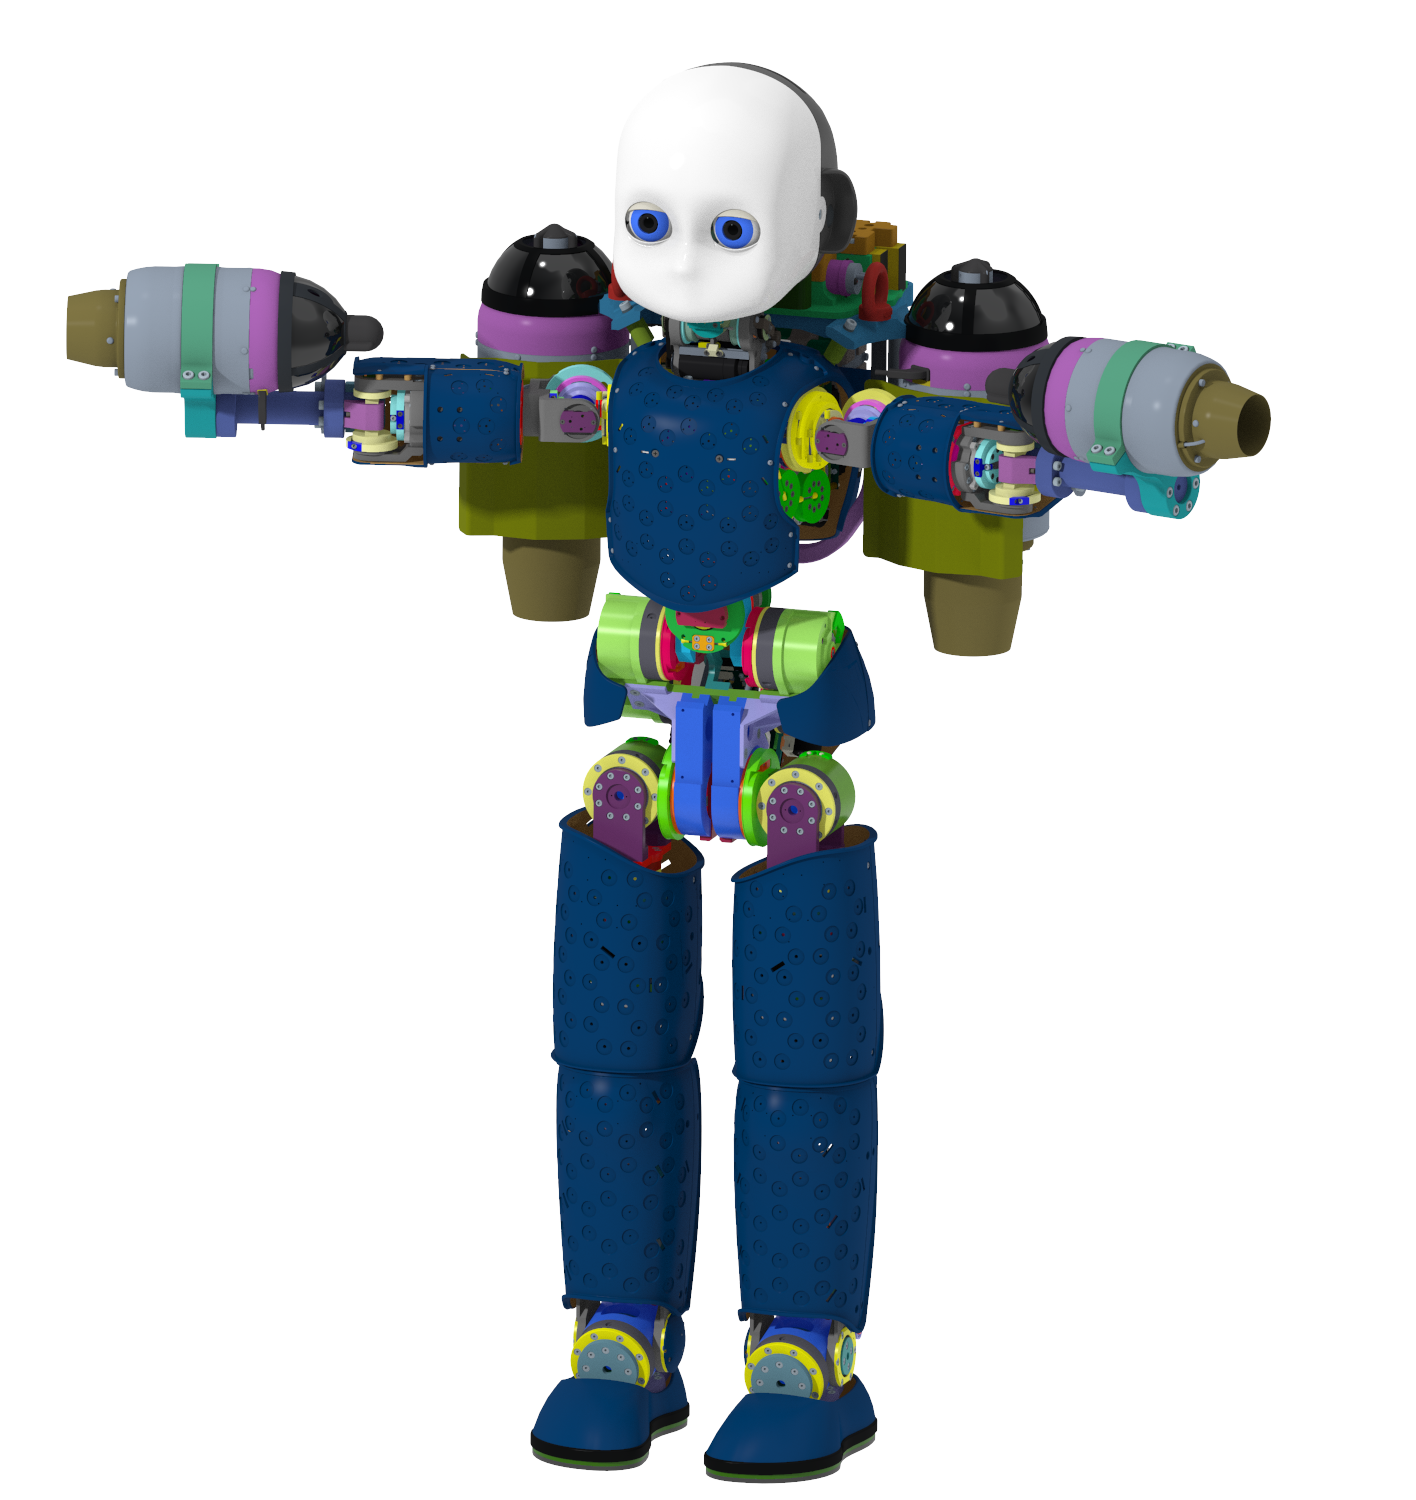
\includegraphics[width=55mm]{./imagines/mk1-5.png}
      \caption{CAD model of the jet-powered humanoid robot iRonCub.}
      \label{fig:iron_cad}
\end{figure}

%  To allow these robots to effectively operate outdoor, a degree of robustness with respect to environmental conditions is therefore required. 
A common assumption for high DoF VTOL systems is that the vehicle operates at relatively \emph{small speed}, often in indoor environments \cite{c8}\cite{c9}\cite{c10}, correspondingly the aerodynamic forces acting on the system are usually negligible and not considered in modeling and control framework \cite{c11}\cite{c28}. When aerodynamic effects are important enough to affect system stability during flight, or high precision is required for performing a task, different modeling and control strategies could be adopted, e.g. to estimate aerodynamic force by designing a momentum-based observer or other disturbances estimation strategies \cite{c17}\cite{c16}, and to compensate estimated aerodynamic force by means of adaptive control strategies \cite{c14}\cite{c15}. However, the absence of an explicit model of the aerodynamic forces could impair the effectiveness of these methods for exploiting physical properties that are beneficial for flight.\looseness=-1

%In several studies, aerodynamic effects are commonly neglected due to the complexity of the aerodynamic model of UAVs and safe flight condition, e.g. \cite{c8}\cite{c9}\cite{c10}. 
%
%Control designs employed to compensate neglected aerodynamic effects and other external disturbances are developed, e.g. a momentum-based compensation of external wrench in \cite{c17}, adaptive controls in \cite{c14}\cite{c15}, or disturbance estimation in \cite{c16}. 

% Aerodynamic forces are often taken into account for performing \emph{aggressive maneuvers} such as spins or flips \giusesays{The previous sentence could aggressively fly away}. 
High-speed flight can benefit from the presence of lift forces that alleviate the effort made by the propellers for gravity compensation. The VTOL dynamical model, in this case, explicitly includes aerodynamic forces \cite{c18}. Few examples include the analysis of blade flapping on quadrotors, modeling first-order aerodynamic effects and evaluating the effect of drag force on thrust power under hovering, \cite{c7}\cite{c20}\cite{c19}.
%
%A brief introduction to feedback control of underactuated VTOL UAVs can be found in , in which system modeling of underactuated VTOLs with aggressive maneuvers like spins and flips, or high-speed flight introduces aerodynamic forces as part of the external forces acting on the vehicle.
%
%Seeking of well-modeled flight systems of VTOLs that work at higher speeds and in outdoor flight with flight characteristics strongly impacted by aerodynamic effects, several works are done, e.g. analysis of blade flapping on quadrotors in \cite{c7}, first-order aerodynamic effects in \cite{c20}, and effects of drag and thrust power under hovering in \cite{c19}. 
%
However, the shape of aerial vehicles has a significant role in modeling aerodynamics effects. It is difficult to design an effective aerodynamic model in case of complex-shaped, high DoF aerial systems \cite{c6}\cite{c18}.

%However, for vehicles that are designed to take advantage of strong aerodynamic lift forces, evaluating drag and lift force models separately is even more complex. A good understanding of aerodynamic effects is useful for evaluating the performance and robustness of current controller but not necessary for developing control algorithm, however, the less of aerodynamic models in control design requires a well-designed feedback control which guarantees the performance with respect to (w.r.t.) the model inaccuracies \cite{c18}. 
%
%The shape of aerial vehicles has a significant role in aerodynamic modeling process. A complex-shaped aerial vehicle leads to the difficulties in mesh generating for CFD analysis and building approximated analytical models with proper defined parameters. This paper thus represents possible methods to overcome these limits.
%  or \emph{flight envelope}. Numerical methods such as  allow to simulate the air-flow conditions on the body by resolving Navier-Stokes equations numerically. 

Different techniques have been developed to properly estimate aerodynamic forces for complex-shaped systems, e.g. wind tunnel test and Computational Fluid Dynamics (CFD) analysis. However, to estimate the aerodynamic forces for an entire set of robot operating conditions, i.e. \emph{flight envelope}, requires to collect a very large number of data. An alternative is to design simpler analytical models via limited dataset provided by wind tunnel tests or CFD simulations. Many of these analytical models assume that the robot body is axisymmetric \cite{c3}\cite{c23}\cite{c25}.  %More general models have been defined which are also valid for non-axisymmetric 3D bluff bodies \cite{c3}.

%i.e. the so-called aerodynamic modeling process based on the measured data from the aforementioned two methods is widely implemented in the flight system design of the aerial vehicles. Many researches about aerodynamic modeling on axisymmetric vehicles have been carried out in the past few years e.g. \cite{c23}\cite{c25} with the parameters (e.g. relative angles) and coordinate systems defined according to vehicles' geometrical characteristics but the methods cannot be applied to a non-axisymmetric 3D bluff body. A more general method introduced in \cite{c3} for defining relative angles allows one to fix the relative orientation between the flow and a random 3D body.

%Many studies and techniques are developed for evaluating the aerodynamic effects acting on aerials vehicles, e.g. the wind tunnel test which measures the air velocity, pressure distributions and aerodynamic forces or CFD analysis that uses numerical analysis to simulate the flow condition. 

%CFD analysis or wind tunnel measurements help researchers to estimate the aerodynamic effects under a given flight envelope (flight velocity and relative angles), however, they do not provide analytical expressions of aerodynamic characteristics (AC) \cite{c3} which are significant for system modeling with aerodynamic effects considered and control design. Thus, the use of simple analytical models of AC, i.e. the so-called aerodynamic modeling process based on the measured data from the aforementioned two methods is widely implemented in the flight system design of the aerial vehicles. Many researches about aerodynamic modeling on axisymmetric vehicles have been carried out in the past few years e.g. \cite{c23}\cite{c25} with the parameters (e.g. relative angles) and coordinate systems defined according to vehicles' geometrical characteristics but the methods cannot be applied to a non-axisymmetric 3D bluff body. A more general method introduced in \cite{c3} for defining relative angles allows one to fix the relative orientation between the flow and a random 3D body.
%  The proposed flight envelopes consider the robot moving at high speed, in presence of wind and wind gusts.

In this paper we propose a framework to include aerodynamic forces in the modeling and control design of high DoF VTOL systems, which in the case under study are represented by the flying humanoid robot iRonCub. 
%
To improve the iRonCub operativity in presence of aerodynamic effects, we applied the following procedure. At first, a series of CFD simulations is performed on a simplified robot model, in order to generate a dataset of the aerodynamic forces acting on the robot for a given flight envelope. Secondly, a model for a non-axisymmetric bluff body is designed to fit the collected dataset and estimate the aerodynamic characteristics in between the flight envelope. The model is verified to be also physically consistent (positivity of the Drag coefficient). Finally, the designed model is used to improve the iRonCub flight-control strategy developed in our previous works \cite{c1}\cite{c2} by compensation of the aerodynamic forces via \emph{feedback linearization} and improvement of the controller robustness with \emph{gain scheduling}.

%Concerning a flying humanoid robot as a highly complex-shaped and underactuated VTOL UAV which explores high-speed flight in outdoor environment with a possible wind gust impact, understanding aerodynamic effects plays a significant role not only for performance evaluation but also for control design due to strong unavoidable perturbations. This paper, thus, represents aerodynamic modeling on a non-axisymmetric 3D bluff body \cite{c26} as the flying humanoid robot - iRonCub \cite{c27} platform (see Fig. \ref{fig:iron_cad}) based on the CFD simulation data implementing the definition of relative angles introduced in \cite{c3}. Instead of evaluating lift and drag for the vehicles as designed for taking advantages from lift, the aerodynamic force acting on a non-aerodynamic shape as iRonCub is simply decomposed w.r.t. a defined frame and no lift force is specified in this case. The identified aerodynamic models are then used for analyzing the robustness of the current controller and applied on the control level to improve the current controller towards aerodynamic effects. 

The paper is organized as follows. Sec.~\ref{background} recalls notation, system modeling and fundamentals of aerodynamic modeling. In Sec.~\ref{methods}, we describe the CFD analysis on a simplified iRonCub model and the identification of the aerodynamic characteristics. Sec.~\ref{sec:control} presents the improvements of iRonCub flight controller to handle aerodynamic effects. Simulation results are displayed in Sec.~\ref{simulation}. Sec.~\ref{conclusion} concludes the paper and points out future directions.

